\documentclass[aspectratio=169, pdf, 8pt, unicode]{beamer}
\usepackage[american,russian]{babel}
\usepackage[default]{sourcesanspro}
\usepackage{systeme}
\usepackage{float}
\usepackage{graphicx}
\usepackage{pgfplotstable}
\usepackage{caption}
\usepackage{amsmath}
\usepackage{amssymb}
\usepackage{setspace}
\usepackage{fancyvrb}
\usepackage{outlines}
\usepackage{amsmath,amssymb}
\usepackage{graphicx}
\usepackage{subcaption}
\usepackage{listings}
\usepackage{color}

\definecolor{mygreen}{rgb}{0,0.6,0}
\definecolor{mymauve}{rgb}{0.58,0,0.82}

\DeclareCaptionLabelFormat{gostfigure}{Рисунок #2}
\captionsetup[table]{labelsep=endash,justification=justified,singlelinecheck=false,font=normalsize,skip=0pt}
\captionsetup[figure]{labelformat=gostfigure,labelsep=endash,justification=centering,singlelinecheck=false,font=normalsize}
\pgfplotsset{compat=1.9}

\mode<presentation> {
\usetheme{Madrid}
}

\setbeamerfont{institute}{size=\normalsize}
\setbeamertemplate{itemize/enumerate body begin}{\large}
\setbeamertemplate{itemize/enumerate subbody begin}{\tiny}

\title[Программирование на необитаемом острове]{Программирование на необитаемом острове}

\author{Микоян Филипп}

\institute[МФТИ]{
    Московский физико-технический институт (национальный исследовательский университет)
}

\date{}

\setbeamertemplate{caption}[numbered]

\begin{document}

\lstdefinelanguage{AVR}{
morekeywords=[1]{adc,add,adiw,sub,subi,sbc,sbiw,and,andi,or,ori,eor,com,
                neg,sbr,cbr,inc,dec,tst,clr,ser,mul,muls,mulsu,fmul,fmuls,
                fmulsu,rjmp,ijmp,eijmp,jmp,rcall,icall,eicall,call,ret,
                reti,cpse,cp,cpc,cpi,sbrc,sbrs,sbic,sbis,brbs,brbc,breq,
                brne,brcs,brcc,brsh,brlo,brmi,brpl,brge,brlt,brhs,brhc,
                brts,brtc,brvs,brvc,brie,brid,mov,movw,ldi,lds,ld,ldd,st,
                sts,std,lpm,elpm,spm,in,out,push,pop,lsl,lsr,rol,ror,asr,
                swap,bset,bclr,sbi,cbi,bst,bld,sec,sen,cln,sez,clz,sei,cli,
                ses,cls,sev,clv,set,clt,seh,clh,break,nop,sleep,wdr},%
morekeywords=[2]{X,Y,Z,r0,r1,r2,r3,r4,r5,r6,r7,r8,r9,r10,r11,r12,r13,r14,
                r15,r16,r17,r18,r19,r20,r21,r22,r23,r24,r25,r26,r27,r28,r29,
                r30,r31,tccr3a,tccr3b,tcnt3h,tcnt3l,ocr3ah,ocr3al,ocr3bh,
                ocr3bl,icr3h,icr3l,etimsk,etifr,pcmsk1,pcmsk0,clkpr,sreg,
                sph,spl,ucsr1c,ubrr1h,eimsk,gimsk,gicr,gifr,timsk,tifr,
                spmcr,emcucr,mcucsr,tccr0,tcnt0,ocr0,sfior,tccr1a,tccr1b,
                tcnt1h,tcnt1l,ocr1ah,ocr1al,ocr1bh,ocr1bl,tccr2,assr,icr1h,
                icr1l,tcnt2,ocr2,wdtcr,ubrrhi,ucsroc,ubrroh,eearh,eearl,
                eedr,eecr,porta,ddra,pina,portb,ddrb,pinb,portc,ddrc,pinc,
                portd,ddrd,pind,spdr,spsr,spcr,udr0,udr,ucsr0a,usrucsr0b,ucr,
                ubrr0,ubrr0l,ubrr,acsr,porte,ddre,pine,osccal,udr1,ucsr1a,
                ucsr1b,ubrr1,ubrr1l,com3a1,com3a0,com3b1,com3b0,foc3a,foc3b,
                wgm31,wgm30,icnc3,ices3,wgm33,wgm32,cs32,cs31,cs30,icf3,
                ocf3a,ocf3b,tov3,pcint15,pcint14,pcint13,pcint12,pcint11,
                pcint10,pcint9,pcint8,pcint7,pcint6,pcint5,pcint4,pcint3,
                pcint2,pcint1,pcint0,CLKPCE,CLKPS3,CLKPS2,CLKPS1,CLKPS0,INT1,
                INT0,INT2,PCIE1,PCIE0,IVSEL,IVCE,INTF1,INTF0,INTF2,PCIF1,PCIF0,
                TOIE1,OCIE1A,OCIE1B,OCIE2,TICIE1,TOIE2,TOIE0,OCIE0,TOV1,OCF1A,
                OCF1B,OCF2,ICF1,TOV2,TOV0,OCF0,SPMIE,RWWSB,ASB,RWWSRE,ASRE,
                BLBSET,PGWRT,PGERS,SPMEN,SM0,SRL2,SRL1,SRL0,SRW01,SRW00,SRW11,
                ISC2,SRE,SRW,SRW10,SE,SM,SM1,ISC11,ISC10,ISC01,ISC00,JTD,SM2,
                JTRF,WDRF,BORF,EXTRF,PORF,FOC0,WGM00,PWM0,COM01,COM00,WGM01,
                CTC0,CS02,CS01,CS00,TSM,XMBK,XMM2,XMM1,XMM0,PUD,PSR2,PSR10,PSR1,
                PSR0,COM1A1,COM1A0,COM1B1,COM1B0,FOC1A,FOC1B,PWM11,WGM11,PWM10,
                WGM10,ICNC1,ICES1,CTC11,WGM13,CTC10,WGM12,CTC1,CS12,CS11,CS10,
                FOC2,WGM20,PWM2,COM21,COM20,WGM21,CTC2,CS22,CS21,CS20,AS2,
                TCN2UB,OCR2UB,TCR2UB,WDTOE,WDCE,WDE,WDP2,WDP1,WDP0,EERIE,EEMWE,
                EEWE,EERE,PORTA7,PORTA6,PORTA5,PORTA4,PORTA3,PORTA2,PORTA1,PORTA0,
                DDA7,DDA6,DDA5,DDA4,DDA3,DDA2,DDA1,DDA0,PINA7,PINA6,PINA5,PINA4,
                PINA3,PINA2,PINA1,PINA0,PORTB7,PORTB6,PORTB5,PORTB4,PORTB3,PORTB2,
                PORTB1,PORTB0,DDB7,DDB6,DDB5,DDB4,DDB3,DDB2,DDB1,DDB0,PINB7,PINB6,
                PINB5,PINB4,PINB3,PINB2,PINB1,PINB0,PORTC7,PORTC6,PORTC5,
                PORTC4,PORTC3,PORTC2,PORTC1,PORTC0,DDC7,DDC6,DDC5,DDC4,
                DDC3,DDC2,DDC1,DDC0,PINC7,PINC6,PINC5,PINC4,PINC3,PINC2,
                PINC1,PINC0,PORTD7,PORTD6,PORTD5,PORTD4,PORTD3,PORTD2,
                PORTD1,PORTD0,DDD7,DDD6,DDD5,DDD4,DDD3,DDD2,DDD1,
                DDD0,PIND7,PIND6,PIND5,PIND4,PIND3,PIND2,PIND1,PIND0,
                PORTE2,PORTE1,PORTE0,DDE2,DDE1,DDE0,PINE2,PINE1,PINE0,
                RXC,TXC,UDRE,FE,OR,U2X,RXC0,TXC0,UDRE0,FE0,OR0,DOR0,
                PE0,U2X0,MPCM0,RXC1,TXC1,UDRE1,FE1,OR1,DOR1,PE1,U2X1,
                MPCM1,SPIE,SPE,DORD,MSTR,CPOL,CPHA,SPR1,SPR0,SPIF,WCOL,SPI2X,
                RXCIE,TXCIE,UDRIE,RXEN,TXEN,CHR9,UCSZ2,RXB8,TXB8,RXCIE0,TXCIE0,
                UDRIE0,RXEN0,TXEN0,CHR90,UCSZ02,RXB80,TXB80,RXCIE1,TXCIE1,
                UDRIE1,RXEN1,TXEN1,CHR91,UCSZ12,RXB81,TXB81,URSEL0,UMSEL0,
                UPM01,UPM00,USBS0,UCSZ01,UCSZ00,UCPOL0,URSEL1,UMSEL1,UPM11,
                UPM10,USBS1,UCSZ11,UCSZ10,UCPOL1,ACD,AINBG,ACBG,ACO,ACI,ACIE,
                ACIC,ACIS1,ACIS0,BLB12,BLB11,BLB02,BLB01,XL,XH,YL,YH,ZL,
                ZH,RAMEND,EEPROMEND,FLASHEND,SMALLBOOTSTART,SECONDBOOTSTART,
                THIRDBOOTSTART,LARGEBOOTSTART,BOOTSTART,PAGESIZE,INT0addr,
                INT1addr,INT2addr,PCINT0addr,PCINT1addr,TIMER3CAPTaddr,
                TIMER3COMPAaddr,TIMER3COMPBaddr,TIMER3OVFaddr,TIMER2COMPaddr,
                TIMER2OVFaddr,TIMER1CAPTaddr,TIMER1COMPAaddr,TIMER1COMPBaddr,
                TIMER1OVFaddr,TIMER0COMPaddr,TIMER0OVFaddr,SPISTCaddr,
                USART0RXCaddr,USART1RXCaddr,USART0UDREaddr,USART1UDREaddr,
                USART0TXCaddr,USART1TXCaddr,EE_RDYaddr,ANA_CMPaddr,
                SPM_RDYadd,mcucr,ubrr0h,ucsr0c,ucsr0b},%
morekeywords=[3]{org,def,equ,db,include,dseg,cseg,eseg},%
sensitive=f,%
morecomment=[l];,%
}[keywords,comments,strings]%



\begin{frame}[fragile]
\titlepage
\vspace*{-1cm}
\begin{figure}[H]
	\centering
	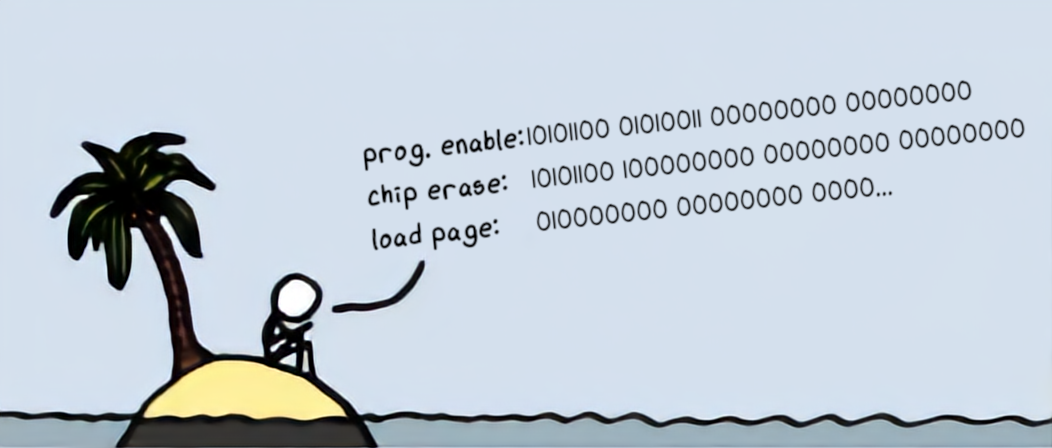
\includegraphics[width=0.6\textwidth]{resources/xkcd.png}
	\caption{Вольная интерпретация комикса xkcd}
\end{figure}
\end{frame}

\begin{frame}[fragile]
\frametitle{}
	\begin{figure}[H]
	      \centering
	      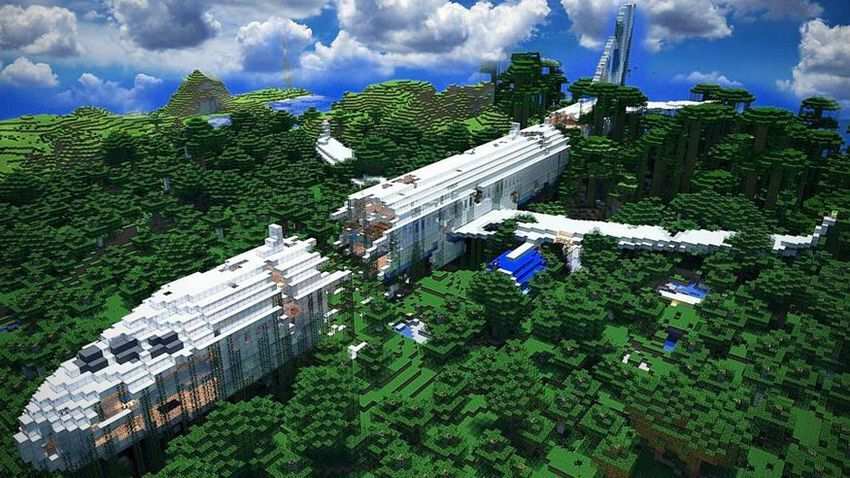
\includegraphics[width=0.6\textwidth]{resources/minecraft_plane.jpg}
	      \caption{Итак, ваш самолёт разбился...}
	\end{figure}
\end{frame}

\begin{frame}[fragile]
\frametitle{Что у нас есть в наличии?}
	\begin{outline}
		\1 Дикие лимоны
		\1 Самолётная фара и высоковольтный аккумулятор для неё (в нашем случае лампочка накаливания)
		\1 Спичечный коробок с:
			\2 { \normalsize Микроконтроллером AVR Attiny13 }
			\2 { \normalsize Несколькими проводами }
			\2 { \normalsize Парой кнопок }
	\end{outline}
	Попробуем собрать из этого аварийный маяк, мигающий с периодом 1 секунда.
	\begin{figure}[H]
		\begin{subfigure}{0.25\textwidth}
			\centering
			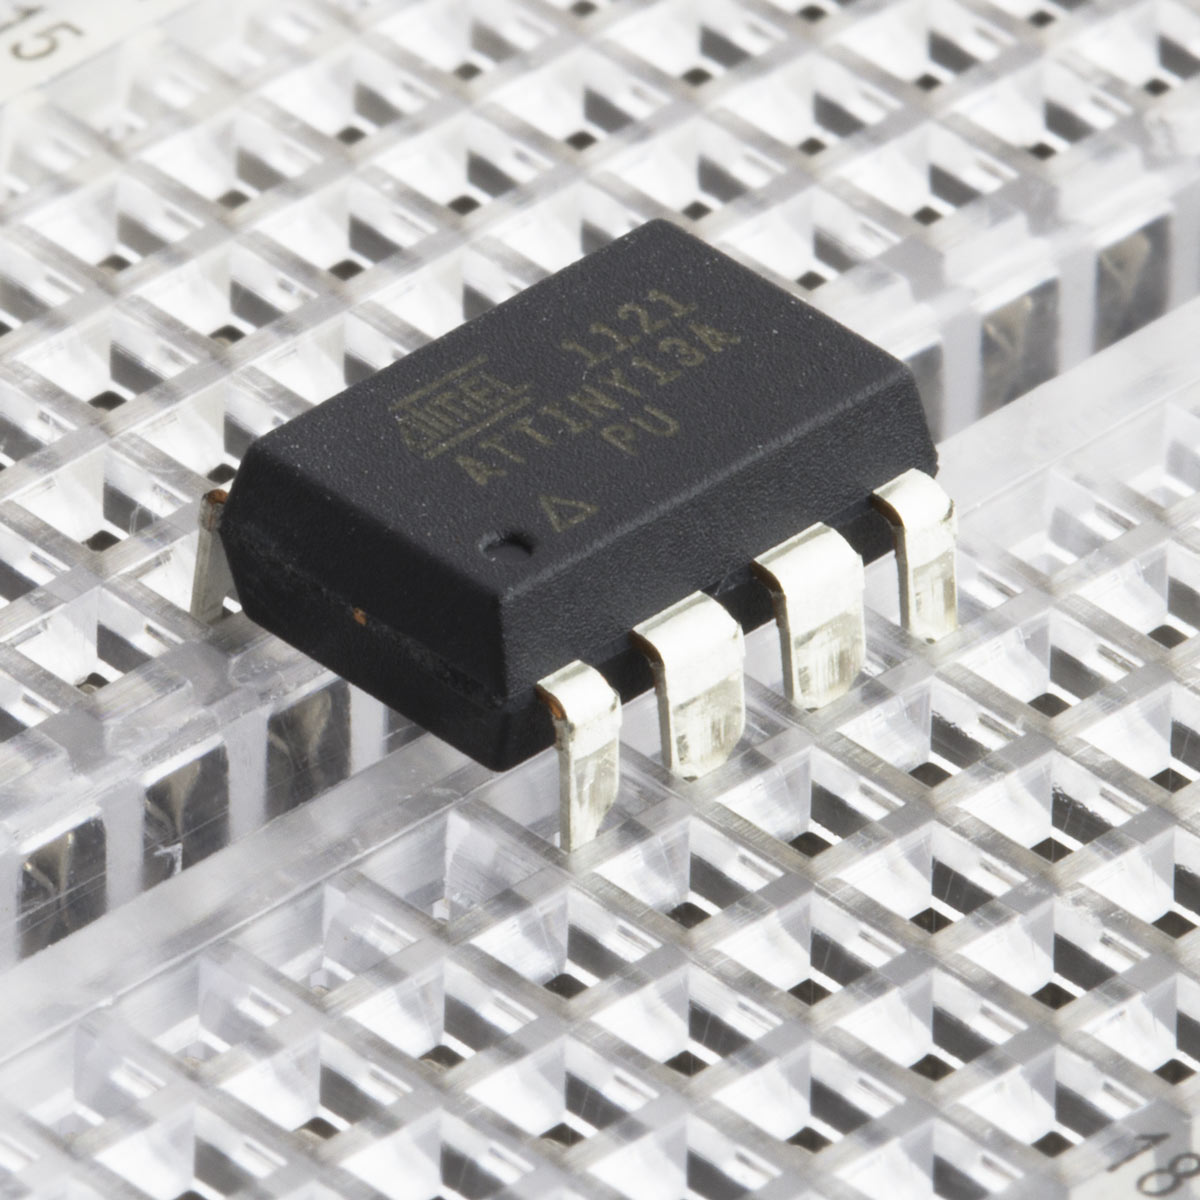
\includegraphics[width=\textwidth]{resources/attiny13a.JPG}
			\caption{Микроконтроллер ATtiny13A}
		\end{subfigure}
		\begin{subfigure}{0.35\textwidth}
			\centering
			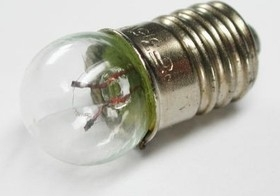
\includegraphics[width=\textwidth]{resources/lamp.jpg}
			\caption{Релейный модуль для макетных плат}
		\end{subfigure}
	\end{figure}
\end{frame}

\begin{frame}[fragile]
	\begin{figure}[H]
		\centering
		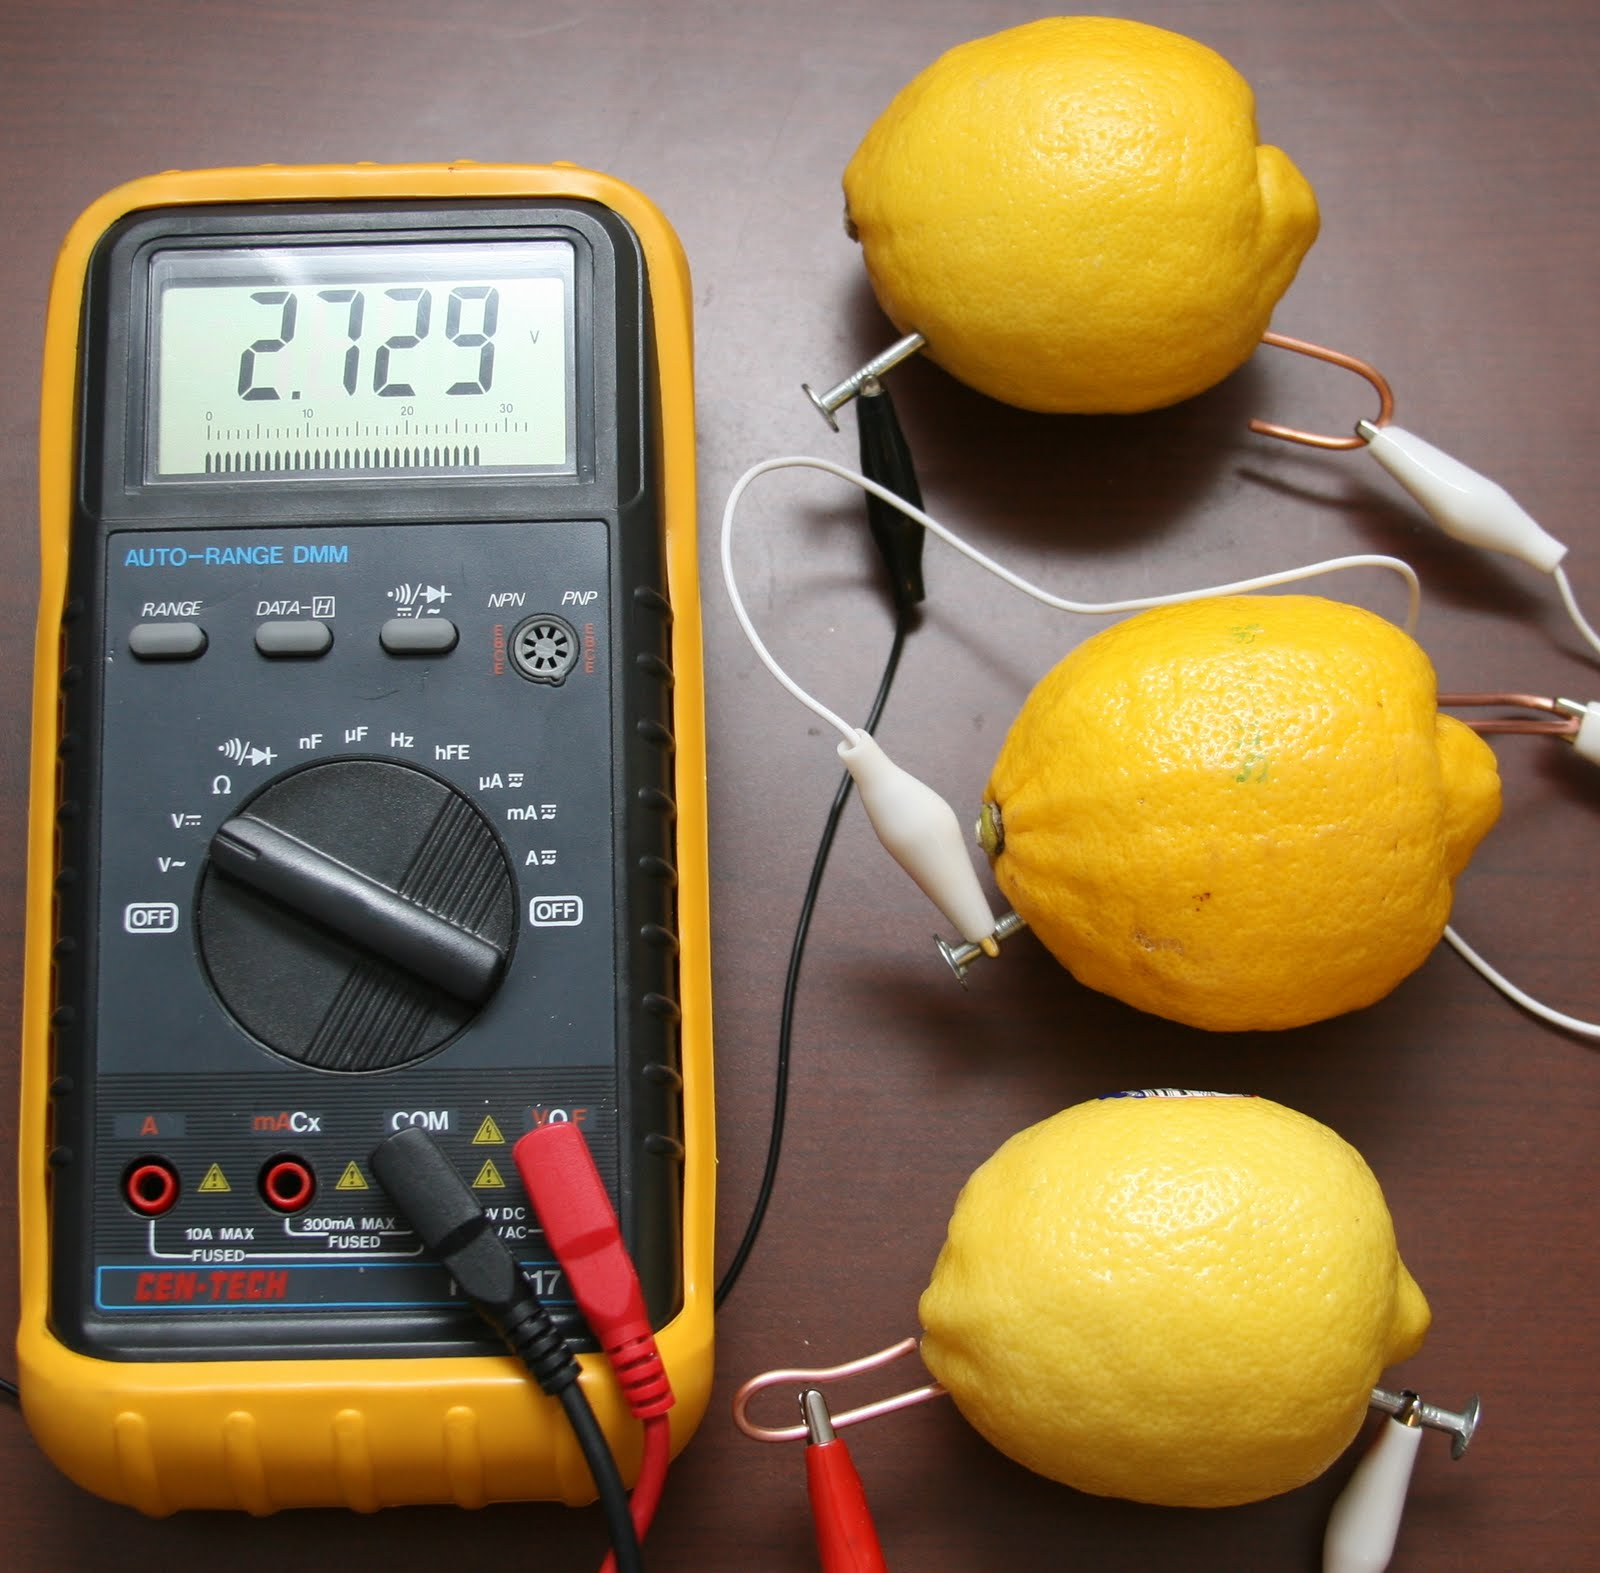
\includegraphics[width=0.4\textwidth]{resources/lemons.jpg}
		\caption{Лимонная кислота\ \cyrdash\ электролит. С каждого лимона получаем почти 1В}
	\end{figure}
\end{frame}

\begin{frame}[fragile]
\frametitle{План действий}
	\begin{itemize}
		\item Написать на Паскале программу, которая сможет ждать полсекунды.
		\item Переписать её на ассемблер.
		\item Добавить в программу мигание светодиодом.
		\item Понять, как она представляется в машинных кодах.
		\item Прочитать, какими командами её можно записать в память микроконтроллера.
		\item Изучить протокол \texttt{SPI} передачи данных.
		\item Прошить микроконтроллер.
	\end{itemize}
	\begin{figure}[H]
		\centering
		\vspace*{-0.5cm}
		
\includegraphics[width=0.32\textwidth]{resources/kitty_rus.jpg}
	\end{figure}
\end{frame}

\begin{frame}[fragile]
\frametitle{Как микроконтроллеру ждать полсекунды?}
	{ \large
		Микроконтроллер\ 'ждёт', исполняя инструкции. Исполнение одной инструкции занимает какое-то время,
		определяемое частотой работы микроконтроллера(\textbf{тактовой частотой}) и числом тактов, необходимых на
		исполнение инструкции. Имеем систему:
		$$
		\begin{cases}
			f = 128\ \text{КГц} = 128\ 000 \text{ тактов в секунду } & \text{\cyrdash\ тактовая частота микроконтроллера} \\
			T/2 = 0.5\text{ секунды } & \text{\cyrdash\ необходимое время ожидания} \\
			N = (T/2) \cdot f = 64\ 000 & \text{\cyrdash\ тактов нужно подождать} \\
		\end{cases}
		$$
		\begin{figure}[H]
			\centering
			\vspace*{-0.5cm}
			
\includegraphics[width=0.32\textwidth]{resources/counting.jpg}
		\end{figure}
		\vspace*{-0.2cm}
		Вопрос: а какова тактовая частота процессора в вашем персональном компьютере?
	}
\end{frame}

\begin{frame}[fragile]
\frametitle{За сколько тактов процессора исполняется данная программа?}
	\begin{figure}[!htb]
		\centering
		\lstset{language=Pascal,
			keywordstyle=\color{blue}\bfseries,
			numberstyle=\color{mymauve},
			inputencoding=utf8,
			escapeinside={\%*}{*)},
			morecomment=[l]{//},
			frame=leftline}
		\begin{minipage}{.40\textwidth}
			\begin{lstlisting}
// %*Эта программа уменьшает значение*)
// %*переменной 'a' от десяти до нуля,*)
// %*т.е. считает до десяти.*)
var
    a: integer;

begin
    a := 10;
    repeat
        a := a - 1;
    until a = 0;
end.

			\end{lstlisting}
		\end{minipage}
		\begin{minipage}{.55\textwidth}
			\begin{lstlisting}
// %*Та же самая программа,*)
// %*но использует goto и dec*)
var
    a: integer;

label
    loop;

begin
    a := 10;
loop:
    dec(a); // %*идентично*) a = a - 1;
            // Dec = Decrement = %*уменьшить на 1*)
    if (NOT (a = 0)) then
        goto loop;
end.
			\end{lstlisting}
		\end{minipage}
	\end{figure}
		В процессоре нашего микроконтроллера \texttt{dec()} выполняется ровно за один такт процессора.
		Проверка условия в \texttt{if} и \texttt{goto} тоже тратят на исполнение по одному такту. Таким образом, для
		исполнения данного цикла с $N$ итерациями требуется $3*N$ тактов. В данном случае 30.
\end{frame}

\begin{frame}[fragile]
\frametitle{Сколько нужно регистров, чтобы написать такой длинный цикл?}
	{ \large
		Итак, чтобы подождать полсекунды, нужно прокрутить $64\ 000$ тактов процессора, а так как каждая итерация
		исполняется за $3$ такта, цикл придётся написать на $\frac{64\ 000}{3} \approx 21500$ итераций.

		Проблема в том, что в микроконтроллере переменные процессора\ \cyrdash\ \textbf{регистры}\ \cyrdash\ занимают
		всего один байт и умеют считать только до $256$. Если же их два, то уже можно создать цикл из $256*256=65536$
		итераций.
		\begin{figure}[H]
		      \centering
		      
\includegraphics[width=0.4\textwidth]{resources/sad_kitty_rus.png}
		\end{figure}
	}
\end{frame}

\begin{frame}[fragile]
\frametitle{Как посчитать до $21\ 500$ с двумя байтами?}
		\ \ Программа ниже, имея в распоряжении два байта, считает до двадцати одной тысячи.
		Она уменьшает \texttt{r2} от $255$ до $0$, и, когда эта переменная становится равной нулю,
		уменьшает \texttt{r1} на единичку.

		\ \ Таким образом, каждое уменьшение \texttt{r1}\ \cyrdash\ это $256$ проходов внутреннего цикла.
		В сумме до обнуления \texttt{r1} исполняется $\approx 84*256 \approx 21 500$ итераций внутреннего цикла,
		на что затрачивается $21\ 500 \cdot 3 = 64\ 500$ тактов и что создаёт задержку приблизительно в
		$\frac{64500}{128000} \approx 0.5$ секунды.
		Когда \texttt{r1} обнуляется, программа заканчивает исполнение.
		\lstset{language=Pascal,
			keywordstyle=\color{blue}\bfseries,
			numberstyle=\color{mymauve},
			inputencoding=utf8,
			escapeinside={\%*}{*)},
			morecomment=[l]{//},
			frame=leftline}
			\begin{lstlisting}
var r1, r2: byte;

label loop;

begin
    r1 := 83;  // r1 - %*'старший разряд', уменьшается в 256 раз реже, чем r2*)
    r2 := 255; // r2 - %*'младший разряд', постоянно бегает от 255 до 0*)

loop:
    dec(r2);
    if (NOT (r2 = 0)) then
        goto loop;
    dec(r1);
    if (NOT (r1 = 0)) then
        goto loop;
end.
			\end{lstlisting}
\end{frame}

\begin{frame}[fragile]
\frametitle{Для начала перепишем простой цикл на ассемблер}
	\begin{figure}[!htb]
		\centering
		\begin{minipage}{.35\textwidth}
		\lstset{language=Pascal,
			keywordstyle=\color{blue}\bfseries,
			numberstyle=\color{mymauve},
			inputencoding=utf8,
			escapeinside={\%*}{*)},
			morecomment=[l]{//},
			frame=leftline}
			\begin{lstlisting}
var
    a: integer;

label
    loop;

begin
    a := 10;
loop:
    dec(a);
    if (NOT (a = 0)) then
        goto loop;
end.
			\end{lstlisting}
		\end{minipage}
		\begin{minipage}{.55\textwidth}
			\centering
			\lstset{language=AVR,
			keywordstyle=\color{blue}\bfseries,
			numberstyle=\color{mymauve},
			inputencoding=utf8,
			escapeinside={\%*}{*)},
			morecomment=[l]{//},
			frame=leftline}
			\begin{lstlisting}
;   %*Комментарии на ассемблере пишутся так.*)

;   %*В этой программе роль переменной*)
; %*'a' играет регистр 'r20'.*)

    ldi r20, 10 ; r20 := 10;
                ; ldi = LoaD Immediate =
                ; = '%*положить число в регистр*)'
loop:
    dec  r20  ;   %*Вычитает из значения регистра*)
              ; %*единичку и присваивает ему.*)
              ;   %*Если значение стало равно нулю,*)
              ; %*'выставляет' определённый флаг*)
              ; %*Z (Zero) в состоянии процессора.*)

    brne loop ;   %*brne = BRanch Not Equal = прыгни*)
              ; %*на метку, если не равно (нулю).*)
              ;   %*Смотрит, выставлен ли флаг Z.*)
              ; %*Если не выставлен, прыгает на метку,*)
              ; %*иначе ничего не делает.
			\end{lstlisting}
		\end{minipage}
	\end{figure}
\end{frame}

\begin{frame}[fragile]
\frametitle{Теперь посчитаем до двадцати тысяч на ассемблере}
	\begin{figure}[!htb]
		\centering
		\begin{minipage}{.45\textwidth}
		\lstset{language=Pascal,
			keywordstyle=\color{blue}\bfseries,
			numberstyle=\color{mymauve},
			inputencoding=utf8,
			escapeinside={\%*}{*)},
			morecomment=[l]{//},
			frame=leftline}
			\begin{lstlisting}
var r19, r20: byte;

label loop;

begin
    r19 := 83;  // %*старший разряд*)
    r20 := 255; // %*младший разряд*)

loop:
    dec(r20);
    if (NOT (r20 = 0)) then
        goto loop;
    dec(r19);
    if (NOT (r19 = 0)) then
        goto loop;
end.
			\end{lstlisting}
		\end{minipage}
		\begin{minipage}{.45\textwidth}
			\centering
			\lstset{language=AVR,
			keywordstyle=\color{blue}\bfseries,
			numberstyle=\color{mymauve},
			inputencoding=utf8,
			escapeinside={\%*}{*)},
			morecomment=[l]{//},
			frame=leftline}
			\begin{lstlisting}
      ldi  r19, 83  ; r19 := 83;
      ldi  r20, 255 ; r20 := 255;
loop:
      dec  r20
      brne loop
      dec  r19
      brne loop
			\end{lstlisting}
		\end{minipage}
	\end{figure}
\end{frame}

\begin{frame}[fragile]
\frametitle{Научимся менять напряжение на ножке}
	{
		Выставление напряжения на ножке делается очень просто, оно почти ничем не отличается от присваивания значения
		регистру. Микроконтроллер ATtiny13 имеет два особых регистра\ \cyrdash\ \texttt{DDRB} и \texttt{PORTB}.
		Эти регистры\ \cyrdash\ битовые маски, т.е. каждому биту в этих регистрах соответствует своя ножка.

		Например, присвоив число $2 = 0b10 = (1 << 1)$, регистру
		\texttt{DDRB}, можно настроить ножку номер 1 как \texttt{OUTPUT}\ \cyrdash\ выходную. А присвоив число $2$
		регистру \texttt{PORTB}, можно выставить на первой ножке напряжение 5 В.
	}
	\begin{figure}[!htb]
		\centering
		\begin{minipage}{.45\textwidth}
			\centering
			\lstset{language=C++,
			keywordstyle=\color{blue}\bfseries,
			numberstyle=\color{mymauve},
			inputencoding=utf8,
			escapeinside={\%*}{*)},
			morecomment=[l]{//},
			morekeywords={pinMode, digitalWrite, OUTPUT, HIGH},
			title=\text{Код для Ардуино на языке C++},
			frame=leftline}
			\begin{lstlisting}
// %*Настраивает первую ножку на выход*)
// %*(это важно, так как ножки могут*)
// %*также работать на вход)*)
    pinMode(1, OUTPUT);

// %*Выставляет единицу на ножке*)
    digitalWrite(1, HIGH);

// %*Вечный цикл*)
    while (1);
			\end{lstlisting}
		\end{minipage}
		\begin{minipage}{.45\textwidth}
			\centering
			\lstset{language=AVR,
			keywordstyle=\color{blue}\bfseries,
			numberstyle=\color{mymauve},
			inputencoding=utf8,
			escapeinside={\%*}{*)},
			morecomment=[l]{//},
			title=\text{Тот же код на ассемблере},
			frame=leftline}
			\begin{lstlisting}
; %*Инструкция out разрешает только*)
; %*присваивания между регистрами,*)
; %*так что нужно сначала присвоить*)
; %*число обычному регистру, и только*)
; %*потом присвоить особому регистру*)
; %*этот обычный.*)
    ldi r24,  0x02
; %*out присваивает регистрам DDRB и*)
; %*PORTB значение регистра r24, т.е. 0x02*)
    out DDRB,  r24
    out PORTB, r24
; %*rjmp - аналог goto*)
; %*Эта строка эквивалентна вечному циклу*)
    L1: rjmp  L1
			\end{lstlisting}
		\end{minipage}
	\end{figure}
\end{frame}

\begin{frame}[fragile]
	\lstset{language=AVR,
	keywordstyle=\color{blue}\bfseries,
	numberstyle=\color{mymauve},
	inputencoding=utf8,
	escapeinside={\%*}{*)},
	morecomment=[l]{//},
	title=\text{\large Будем очень часто менять напряжение на ножке},
	frame=leftline}
	\begin{lstlisting}
    ldi r24, 0x02  ; r24 := 2
    ldi r25, 0x00  ; r25 := 0
    out DDRB,  r24 ; %*DDRB := r24 := 2, настроить*)
                   ; %*первую ножку как OUTPUT*)
L1:
    out PORTB, r24 ; %*PORTB := r24 := 2, выставить*)
                   ; %*напряжение 5В на первой ножке*)
    out PORTB, r25 ; %*PORTB := r25 := 0, убрать*)
                   ; %*напряжение с первой ножки*)
    rjmp  L1       ; goto L1
	\end{lstlisting}
\end{frame}

\begin{frame}[fragile]
	\lstset{language=AVR,
	keywordstyle=\color{blue}\bfseries,
	numberstyle=\color{mymauve},
	inputencoding=utf8,
	escapeinside={\%*}{*)},
	morecomment=[l]{//},
	title=\text{\large Теперь будем менять напряжение на ножке раз в полсекунды},
	frame=leftline}
	\begin{lstlisting}
    ; %*Исходная настройка*)
    ldi r24, 0x02
    ldi r25, 0x00
    out DDRB,  r24

    ; %*Главный цикл*)
L1:
    out PORTB, r24
    rcall WAIT     ; %*Вызывает функцию WAIT()*)
    out PORTB, r25
    rcall WAIT     ; %*Вызывает функцию WAIT()*)
    rjmp  L1

    ; %*Функция WAIT()*)
WAIT:
    ldi  r19, 83  ; r19 := 83;
    ldi  r20, 255 ; r20 := 255;
loop:
    dec  r20
    brne loop
    dec  r19
    brne loop
    ret ; %*ret = RETurn. Прыгает туда, где был сделан rcall*)
	\end{lstlisting}
\end{frame}

\begin{frame}[fragile]
\frametitle{Как происходит загрузка программы в микроконтроллер?}
	{ \large
	\begin{enumerate}
		\item Передаётся последовательность байт \texttt{Programming Enable}\ \cyrdash\ начать программирование.
		\item Если необходимо, передаётся команда \texttt{Chip Erase}\ \cyrdash\ очистить память микроконтроллера.
		\item Запись программы в память происходит постранично. Страница\ \cyrdash\ последовательность из 16 инструкций.
		      Каждая инструкция занимает два байта, т.е. размер страницы равен $32$ байтам, каждый из которых записывается
		      отдельной командой \texttt{Load Program Memory Page}.
		\item После заполнения страницы она записывается в память командой \texttt{Write Program Memory Page}.
	\end{enumerate}
	}
	\begin{figure}[H]
	      \centering
	      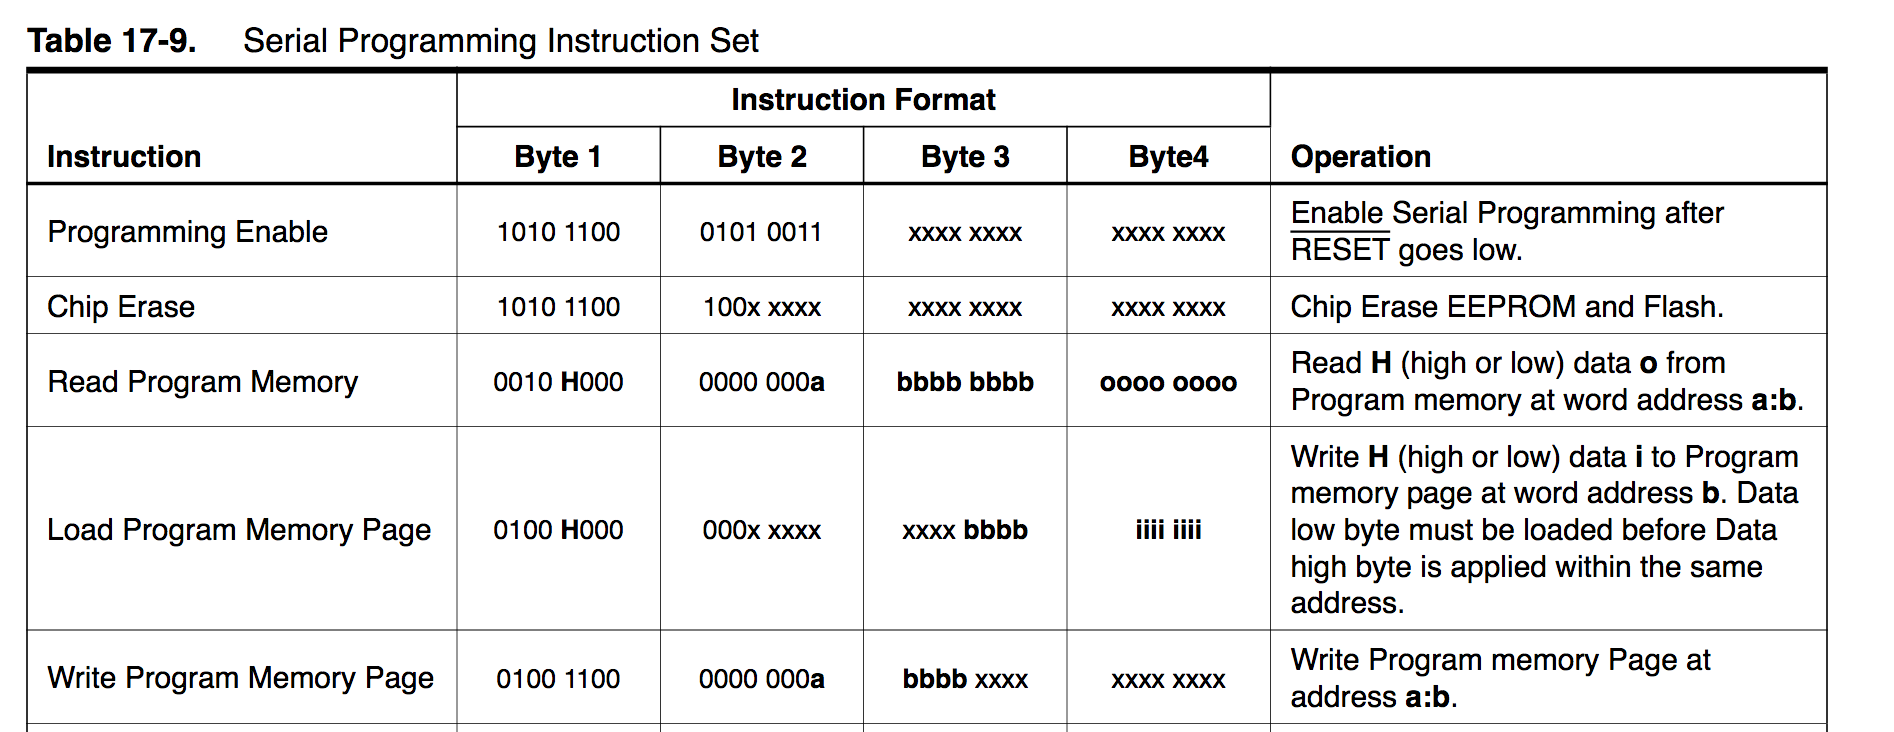
\includegraphics[width=0.6\textwidth]{resources/programming_instruction_set.png}
	      \caption{Скриншот спецификации Atmega13}
	\end{figure}
\end{frame}

\begin{frame}[fragile]
\frametitle{Представление инструкции в машинных кодах}
	\lstset{language=AVR,
	keywordstyle=\color{blue}\bfseries,
	numberstyle=\color{mymauve},
	inputencoding=utf8,
	escapeinside={\%*}{*)},
	morecomment=[l]{//},
	frame=leftline}
	Подробно разребрём процесс записи в память микроконтроллера следующей программы из одной инструкции:
	\begin{lstlisting}
	ldi r19, 0x29
	\end{lstlisting}
	{
		Для начала поймём, что именно мы хотим написать в память. Для этого откроем спецификацию
		языка ассемблера для нашего микроконтроллера:
	}

	\begin{minipage}{.40\textwidth}
		\begin{figure}[H]
		      \centering
		      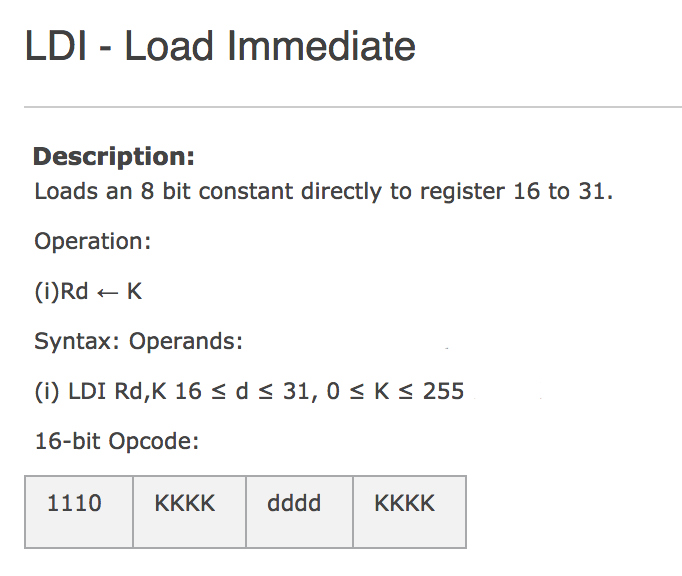
\includegraphics[width=\textwidth]{resources/ldi.png}
		\end{figure}
	\end{minipage}
	\begin{minipage}{.55\textwidth}
		{
			\ \ В спецификации данной инструкции, во-первых, написано, что она делает\ \cyrdash\ загружает восьмибитную
			константу в регистр с номером от \texttt{16} до \texttt{31}. То, что нужно, для регистра \texttt{r19}.

			\ \ Во-вторых, написано, что в качестве аргумента она принимает число \texttt{d}: $16 \leq \texttt{d} \leq 31$
			\ \cyrdash\ номер регистра, младшие четыре бита которого хранятся во втором октете двухбайтной инструкции.
			Ещё одним аргументом является число \texttt{K}: $0 \leq \texttt{K} \leq 255$, которое будет помещено в регистр.
			Его младшие четыре бита располагаются в первом октете инструкции, а старшие четыре бита в третьем октете.
			Четвёртый же октет всегда равен $0b1110$.

			\ \ Используя эту информацию, получим, каким двум байтам соответствует наша инструкция:
			$1110\ 0010\ 0011\ 1001_{2} = E239_{16}$
		}
	\end{minipage}
\end{frame}

\begin{frame}[fragile]
\frametitle{Загрузка инструкции в память микроконтроллера}
	\lstset{language=AVR,
	keywordstyle=\color{blue}\bfseries,
	numberstyle=\color{mymauve},
	inputencoding=utf8,
	escapeinside={\%*}{*)},
	morecomment=[l]{//},
	frame=leftline}
	Итак, мы получили, что нашей инструкции
	\begin{lstlisting}
	ldi r19, 0x29
	\end{lstlisting}
	соответствует пара байт $E239_{16}$. Так как архитектура AVR\ \cyrdash\ little-endian, она хранит\ 'младшие'\
	байты по младшим адресам, и в память нужно поместить выражение $39E2_{16}$, т.е. с поменянными местами байтами.
	Повсеместно используемые архитектуры компании Intel \texttt{i386} и \texttt{x86\_64} тоже являются little-endian
	и хранят данные таким же образом.

	Используя информацию с последних трёх слайдов, запишем последовательность байт, которую нужно подать на микроконтроллер
	для записи в него нашей программы:
	\begin{verbatim}
    10101100 01010011 00000000 00000000 // начать программирование
    10101100 10000000 00000000 00000000 // очистить память

   номер байта       номер инструкции
 внутри инструкции   внутри страницы
        V                 VVVV
    01000000 00000000 00000000 00111001 // загрузить младший байт 0x39 в инструкцию номер 0
    01001000 00000000 00000000 11100010 // загрузить старший байт 0xE2 в инструкцию номер 0
                               ^^^^^^^^
                               сам байт
                 номер страницы
                    V VVVV
    01001100 00000000 00000000 00000000 // записать заполненное выше в страницу номер 0
	\end{verbatim}
\end{frame}

\begin{frame}[fragile]
\frametitle{Что записывать\ \cyrdash\ понятно; а теперь\ \cyrdash\ как записывать?}
	Самый распространённый и простой протокол для прошивки микроконтроллеров AVR\ \cyrdash\ SPI(Serial Peripheral Interface)\ \cyrdash
	\ последовательный периферийный интерфейс. Мы будем использовать следующие три провода:
	\begin{itemize}
		\item \textbf{RESET}\ \cyrdash\ для разрешения прошивки нужно подать на этот провод 0.
		\item \textbf{SCK}\ \cyrdash\ тактовый сигнал, который синхронизирует передачу данных.
		\item \textbf{MOSI}\ \cyrdash\ провод, по которому передаются сами данные.
	\end{itemize}
	На провод \textbf{SCK} подаётся через равные промежутки времени ноль и единица. Частота смена единицы на ноль и обратно определяет
	тактовую частоту шины, определяющую скорость передачи данных. На каждый такт передаётся один бит информации\ \cyrdash\ приёмник
	считывает значение на проводе \textbf{MOSI} в момент, когда значение на \textbf{SCK} меняется с нуля на единицу.
	\begin{minipage}{0.79\textwidth}
		\vspace*{0.3cm}
		\begin{figure}[H]
			\centering
			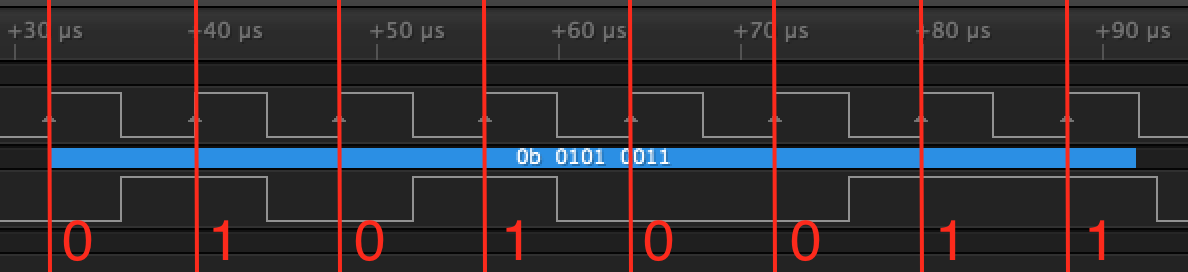
\includegraphics[width=\textwidth]{resources/spi_example.png}
			\caption{Скриншот передачи байта 0b10100011}
		\end{figure}
	\end{minipage}
	\begin{minipage}{0.20\textwidth}
		\vspace*{0.3cm}
		\begin{figure}[H]
			\centering
			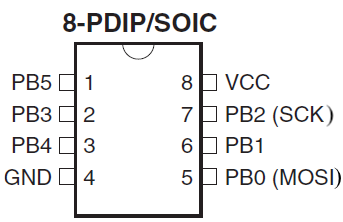
\includegraphics[width=\textwidth]{resources/attiny13_pinout.PNG}
			\caption{Назначение ножек ATtiny13}
		\end{figure}
	\end{minipage}
\end{frame}

\begin{frame}[fragile]
\frametitle{Приступим к сборке схемы?}
	\ \ \ Простой расчёт показывает, что программа для нашего маяка, состоящая из пятнадцати инструкций, занимает
	$(15 \text{ инструкций } * 2 \frac{\text{байт}}{\text{инструкция}}) = 30$ байт. А так как для записи каждого байта
	приходится вводить ещё три байта адресации, да ещё $12$ байт уйдёт на команды включения программирования,
	очищения памяти и записи страницы, в сумме получается $(30 * 4 + 12) = 132 \text{ байта } = 1056 \text{ бит } = 1056$
	нажатий на одну только тактовую кнопку. Времени на это может хватить только на необитаемом острове, к тому же
	вероятность ошибки очень велика.

	\ \ \ Также при сборке схем с кнопками типичной, но сложноустранимой проблемой является \textbf{дребезг контактов}
	\ \cyrdash\ явление, возникающее потому, что в момент нажатия на кнопку контакты в ней из-за упругости
	несколько раз соударяются друг с другом, что приводит к многочисленным, неконтролируемым и очень коротким скачкам
	напряжения. Несмотря на их длительность, даже один скачок может испортить весь процесс прошивки.

	\ \ \ Мы не будем углубляться в теорию методов борьбы с дребезгом\ \cyrdash\ на необитаемом острове можно будет опускать два
	провода в воду, замыкая и размыкая цепь. А на материке мы воспользуемся самосборной схемой, позволяющей\ 'зашивать'
	\ программу по байту за раз. На работу же протокола \texttt{SPI} мы посмотрим с помощью логического анализатора.
	\begin{figure}[H]
		\vspace*{-0.5cm}
		\centering
		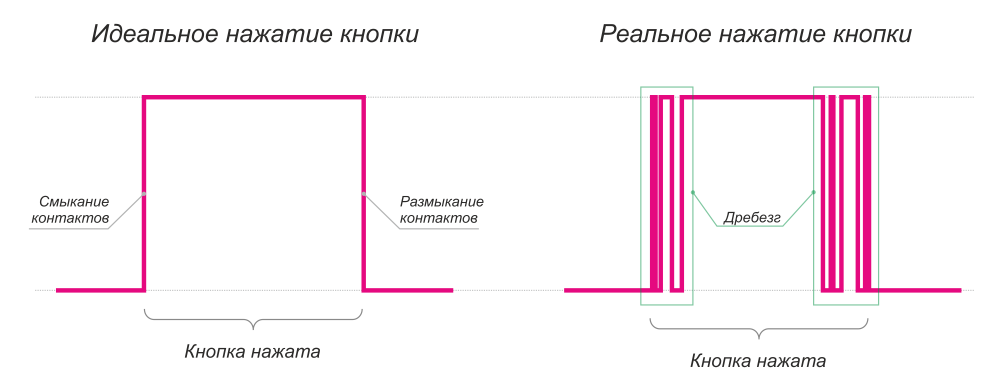
\includegraphics[width=0.4\linewidth]{resources/bounce_rus.png}
		\caption{Дребезг контактов}
	\end{figure}
\end{frame}

\begin{frame}[fragile]
\frametitle{Как это\ \cyrdash\ прошивать по байту за раз?}
	\begin{minipage}{0.54\textwidth}
		\begin{figure}[H]
			\centering
			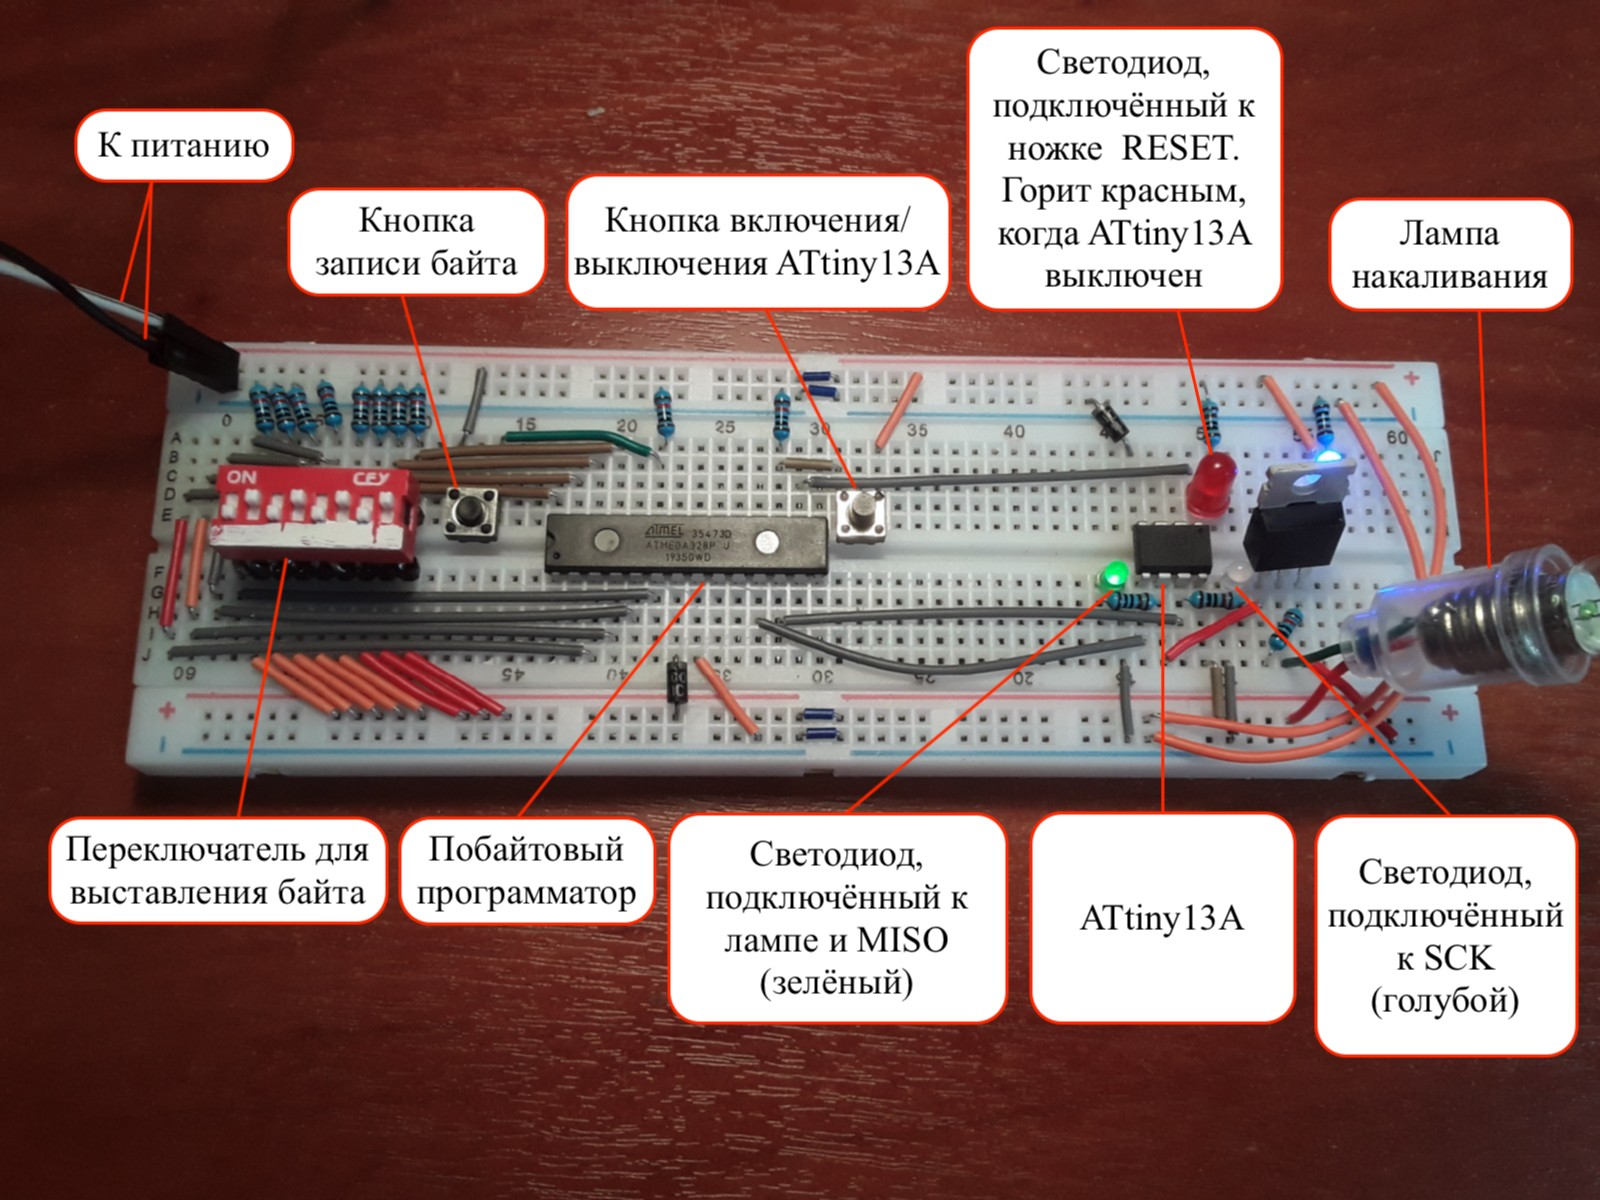
\includegraphics[width=\textwidth]{resources/schematic_new_rus.jpg}
			\caption{Схема для побайтовой прошивки ATtiny13}
		\end{figure}
	\end{minipage}
	\begin{minipage}{0.45\textwidth}
		\vspace*{-0.1cm}
		\begin{itemize}
		\small
			\item \underline{Переключатель}. Ползунки на нём определяют значение байта, который будет отправлен на ATtiny13.
			\item \underline{Кнопка записи}. При нажатии на неё состояния ползунков на переключателях считываются прошивателем
				и отправляются по протоколу SPI на ATtiny13.
			\item \underline{Кнопка RESET}. При нажатии на эту кнопку на ножке RESET ATtiny13 выставляется нулевое
				напряжение, чтобы разрешить программирование. При этом загорается красный светодиод.
			\item \underline{Прошиватель}\ \cyrdash\ микросхема, реализующая всю логику, описанную выше.
			\item \underline{ATtiny13A}. Прошиваемый микроконтроллер.
			\item \underline{Светодиоды MOSI и SCK(голубые)}. Часто мигают, когда происходит передача данных по SPI.
			\item \underline{Светодиод RESET(зелёный)}. Горит, когда на ножке RESET низкое напряжение, т.е. когда возможно
				программирование.
			\item \underline{Светодиод выходной(жёлтый)}. Горит в соответствии с программой на ATtiny13, используется
				при отладке в отсутствие аварийной лампы.
		\end{itemize}
	\end{minipage}
\end{frame}

\begin{frame}[fragile]
\frametitle{Как ещё более ускорить процесс прошивки?}
	{
		\ \ Даже с побайтовым программатором пришлось бы выставлять значения $132^{\underline{\text{х}}}$ байт, поэтому,
		чтобы ещё более ускорить процесс прошивки без потери наглядности, было решено предзагрузить в память программу,
		а вручную переписать лишь одну инструкцию, определяющую частоту мерцания маяка.

		\ \ Так как запись в память микроконтроллера возможна только целой страницей, пришлось немного\ 'разнести'\ программу
		по памяти и добавить ещё одну инструкцию \texttt{rjmp}(\texttt{goto}), которая\ 'перепрыгивает'\ мусор, находящийся в
		конце страницы №1. Переписывать в приведённой ниже программе мы будем только страницу №1.
	}
		\lstset{language=AVR,
		keywordstyle=\color{blue}\bfseries,
		numberstyle=\color{mymauve},
		inputencoding=utf8,
		escapeinside={\%*}{*)},
		morecomment=[l]{//},
		frame=leftline}
		\noindent\makebox[\linewidth]{\rule{\paperwidth}{0.4pt}}
		\begin{minipage}[t]{.32\textwidth}
			\centering
			{ \large \underline{Страница №0} }
			\begin{lstlisting}
; %*Исходная настройка*)
    ldi r24, 0x02
    ldi r25, 0x00
    out DDRB,  r24

; %*Главный цикл*)
L1:
    out PORTB, r24
    rcall WAIT
    out PORTB, r25
    rcall WAIT
    rjmp  L1
			\end{lstlisting}
		\end{minipage}
		\begin{minipage}[t]{.32\textwidth}
			\centering
			{ \large \underline{Страница №1} }
			\begin{lstlisting}
; %*Начало функции WAIT()*)
WAIT:
    ldi  r19, 0x53 ; 83d
    rjmp wait2
			\end{lstlisting}
		\end{minipage}
		\begin{minipage}[t]{.32\textwidth}
			\centering
			{ \large \underline{Страница №2} }
			\begin{lstlisting}
; %*Продолжение функции WAIT()*)
wait2:
    ldi  r20, 255
loop:
    dec  r20
    brne loop
    dec  r19
    brne loop
    ret ; %*конец функции wait*)
			\end{lstlisting}
		\end{minipage}
\end{frame}

\begin{frame}[fragile]
\frametitle{На что будем переписывать страницу №1?}
		\lstset{language=AVR,
		keywordstyle=\color{blue}\bfseries,
		numberstyle=\color{mymauve},
		inputencoding=utf8,
		escapeinside={\%*}{*)},
		morecomment=[l]{//},
		frame=leftline}
		Инструкции в старой версии страницы №1:
		\begin{lstlisting}
    ldi  r19, 0x53 ; 0x53 = 83d
    rjmp wait2     ; rjmp - %*это относительный прыжок. Расстояние до начала след. страницы 14 байт*)
		\end{lstlisting}
		Инструкции в новой версии страницы №1:
		\begin{lstlisting}
    ldi  r19, 0x29 ; 0x29 = 41d, %*в три раза меньше, чем 83d*)
    rjmp wait2
		\end{lstlisting}
		\begin{minipage}{0.49\textwidth}
			\begin{figure}[H]
				\centering
				\includegraphics[width=\textwidth]{resources/rjmp.png}
				\caption{Выдержка из спецификации ассемблера AVR}
			\end{figure}
		\end{minipage}
		\begin{minipage}{0.49\textwidth}
			Для приведённой инструкции \texttt{ldi} мы уже получали представление в машинных кодах
			на предыдущих слайдах: \texttt{0x39E2}.

			Инструкция \texttt{rjmp}, аналог \texttt{goto} из Паскаля, расшифровывается как Relative JuMP\ \cyrdash
			\ относительный прыжок. Это значит, что если аргумент \texttt{rjmp}, например, равен $14_{10} = E_{16}$,
			то управление перенесётся на 15 инструкций вперёд. Об этом написано в спецификации: управление передаётся
			на инструкцию $k + 1$ относительно текущей, где $k$\ \cyrdash\ аргумент \texttt{rjmp}.

			Как видно из спецификации, первые три октета занимает аргумент. Это значит, что в память(с учётом
			little-endian) нужно будет написать \texttt{0x0EC0}.
		\end{minipage}
\end{frame}

\begin{frame}[fragile]
\frametitle{Последовательность байт для прошивки}
	Итак, в память микроконтроллера нужно записать следующую последовательность: \texttt{0x39E20EC0}.

	В соответствии с алгоритмом загрузки программ в память запишем последовательность команд для перезаписи страницы №1.
	Обратите внимание, что в этом случае команда \texttt{chip erase} не подаётся, так как мы хотим переписать только одну страницу.
	\begin{verbatim}
    10101100 01010011 00000000 00000000 // начать программирование

   номер байта       номер инструкции
 внутри инструкции   внутри страницы
        V                 VVVV
    01000000 00000000 00000000 00111001 // загрузить младший байт 0x39 в инструкцию номер 0
    01001000 00000000 00000000 11100010 // загрузить старший байт 0xE2 в инструкцию номер 0

    01000000 00000000 00000001 00001110 // загрузить младший байт 0x0E в инструкцию номер 1
    01001000 00000000 00000001 11000000 // загрузить старший байт 0xC0 в инструкцию номер 1
                               ^^^^^^^^
                               сам байт
                 номер страницы
                    V VVVV
    01001100 00000000 00010000 00000000 // записать заполненное выше в страницу номер 1
	\end{verbatim}
	Всего для перепрошивки микроконтроллера требуется передать на него 24 байта. С этой задачей, благодаря побайтовой записи,
	можно справиться за пару минут.
\end{frame}

\begin{frame}[fragile]
\frametitle{Как прошивать с помощью побайтового программатора?}

	\begin{enumerate}
		\item Вставить белый провод от шнура USB в отверстие рядом с красной дорожкой, а чёрный\ \cyrdash\ в отверстие
			рядом с синей.
		\item Вставить шнур USB в адаптер питания, а тот\ \cyrdash\ в розетку.
		\item Если зелёный светодиод мигает, понаблюдать за ним и на глаз оценить частоту мигания. Он должен мигать
			с периодом примерно одна секунда. Если это не так, нужно \underline{одновременно нажать на обе кнопки}.
		\item Чтобы начать программировать  микроконтроллер, для начала нужно нажать на высокую кнопку подальше
			от переключателей\ \cyrdash\ она выставит низкое напряжение на ножке \texttt{RESET} нашего ATtiny13.
			Загорится красный светодиод. Это значит, можно начинать программирование.
		\item Чтобы\ "отправить"\ на ATtiny13 один байт, нужно выставить его на переключателях(младший бит справа,
			старший слева), затем (при горящем красном светодиоде) нажать на низкую кнопку рядом с переключателем.
			Синяя кнопка мигнёт\ \cyrdash\ это значит, что байт успешно отправлен.
		\item Если в ходе записи совершена ошибка, нажмите два раза на кнопку \texttt{RESET}, чтобы перезагрузить
			микроконтроллер и сбросить записанное.
		\item После окончания программирования нужно нажать на кнопку \texttt{RESET}, чтобы запустить
			перепрограммированный микроконтроллер.
	\end{enumerate}
\end{frame}

\begin{frame}[fragile]
\frametitle{Проверим результат нашей работы}
	\vspace*{0.5cm}
	\begin{figure}[H]
		\centering
		\vspace*{-0.5cm}
		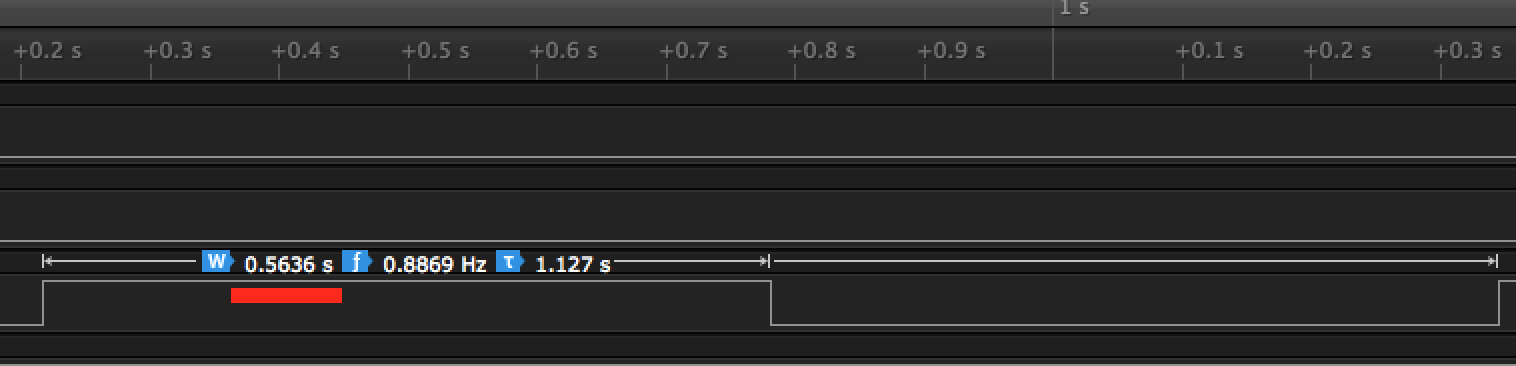
\includegraphics[width=0.6\textwidth]{resources/logic_preloaded.png}
		\caption{Выходной сигнал при исполнении предзагруженной программы. Длина импульсов $0.56$ отличается от
			половины секунды вследствие неточных расчётов и колебаний тактовой частоты.}
	\end{figure}
	\begin{figure}[H]
		\centering
		\vspace*{-0.5cm}
		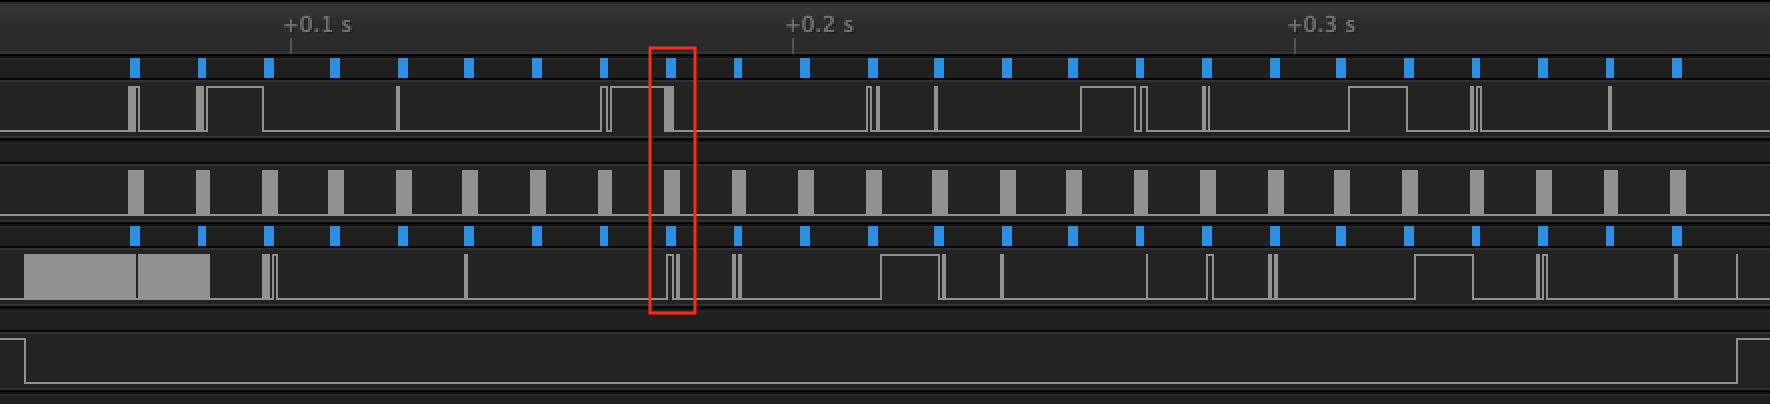
\includegraphics[width=0.6\textwidth]{resources/logic_reprogramming.png}
		\caption{Процесс переписывания страницы №1 микроконтроллера. Каждая синяя полоса\ \cyrdash\ передача одного байта.
		         Очень частые штрихи слева снизу, которые выглядят как сплошная полоса\ \cyrdash\ это мусорный выход с
			 ножки микроконтроллера, когда он уже перезагружен(на ножке \texttt{RESET}), но команда
			 \texttt{Programming Enable} ещё не подана.}
	\end{figure}
\end{frame}

\begin{frame}[fragile]
\frametitle{Проверим результат нашей работы}
	\vspace*{0.5cm}
	\begin{figure}[H]
		\centering
		\vspace*{-0.5cm}
		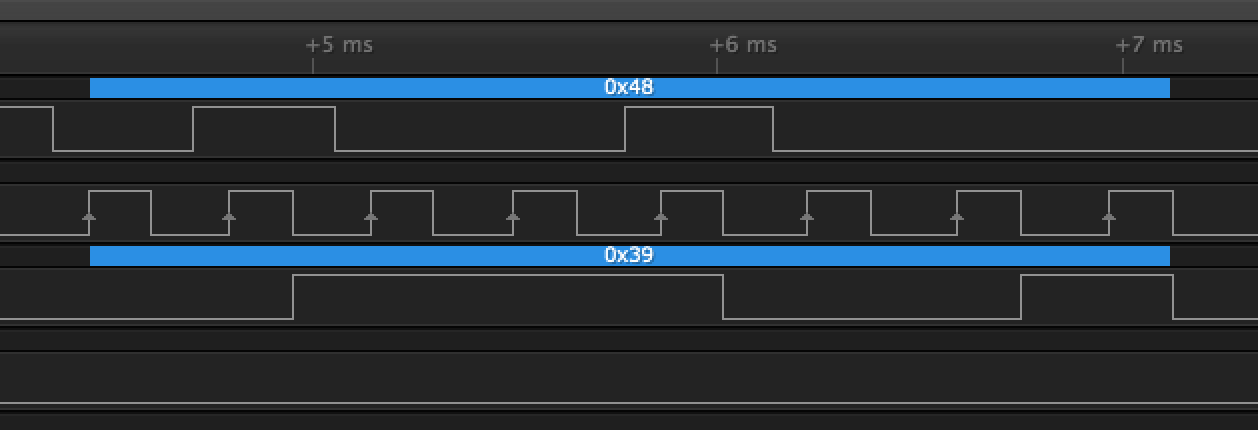
\includegraphics[width=0.5\textwidth]{resources/logic_reprogramming_closeup.png}
		\caption{Передача одного байта в ходе переписывания страницы №1 микроконтроллера. На этом изображении показана
		         часть предыдущего снимка экрана, отмеченная красным прямоугольником. Этот байт, $0x48$\ \cyrdash\ начало
			 загрузки старшего байта инструкции \texttt{ldi r19, 0x29}.  }
	\end{figure}
	\begin{figure}[H]
		\centering
		\vspace*{-0.5cm}
		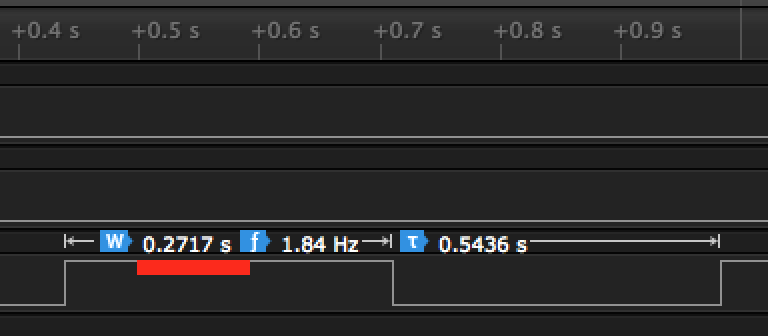
\includegraphics[width=0.3\textwidth]{resources/logic_reprogrammed.png}
		\caption{Выходной сигнал при исполнении модифицированной программы. Длина импульсов $0.27$ отличается от
			$0.56$, как и рассчитывалось, почти в два раза.}
	\end{figure}
\end{frame}

\begin{frame}[fragile]
\frametitle{Напоследок взглянем, как представляется вся программа в машинных кодах}
		\lstset{language=AVR,
		keywordstyle=\color{blue}\bfseries,
		numberstyle=\color{mymauve},
		inputencoding=utf8,
		escapeinside={\%*}{*)},
		morecomment=[l]{//},
		commentstyle=\color{mygreen},
		frame=leftline}
		\noindent\makebox[\linewidth]{\rule{\paperwidth}{0.4pt}}
		\begin{minipage}[t]{.32\textwidth}
			\centering
			{ \large \underline{Страница №0} }
			\begin{lstlisting}
%*; Исходная настройка*)
    ldi r24, 0x02  ; 0x82E0
    ldi r25, 0x00  ; 0x90E0
    out DDRB,  r24 ; 0x87BB

%*; Главный цикл*)
L1:
    out PORTB, r24 ; 0x88BB
    rcall WAIT     ; 0x0BD0
    out PORTB, r25 ; 0x98BB
    rcall WAIT     ; 0x09D0
    rjmp  L1       ; 0xFBCF
			\end{lstlisting}
		\end{minipage}
		\begin{minipage}[t]{.32\textwidth}
			\centering
			{ \large \underline{Страница №1} }
			\begin{lstlisting}
%*; Начало функции WAIT()*)
WAIT:
    ldi  r19, 0x53 ; 0x33E5
    rjmp wait2     ; 0x0EC0
			\end{lstlisting}
		\end{minipage}
		\begin{minipage}[t]{.32\textwidth}
			\centering
			{ \large \underline{Страница №2} }
			\begin{lstlisting}
%*; Продолжение функции WAIT()*)
wait2:
    ldi  r20, 0xFF ; 0x4FEF
loop:
    dec  r20       ; 0x4A95
    brne loop      ; 0xF1F7
    dec  r19       ; 0x3A95
    brne loop      ; 0xE1F7
    ret %*; конец функции wait*)
			\end{lstlisting}
		\end{minipage}
			Опционально: разберём, почему, например, инструкция \texttt{out DDRB, r24} представляется в
			машинных кодах именно так.
\end{frame}

\begin{frame}[fragile]
\frametitle{Чему мы научились?}
	\begin{itemize}
		\item Считать до двадцати тысяч, имея только однобайтные регистры.
		\item Считать до двадцати тысяч на ассемблере.
		\item Мигать светодиодом/аварийным маяком каждые полсекунды на ассемблере.
		\item Переписывать программу с языка ассемблера на машинные коды.
		\item Загружать машинные коды по \texttt{SPI} в память микроконтроллера.
	\end{itemize}
	\begin{figure}[H]
		\centering
		\vspace*{-0.2cm}
		
\includegraphics[width=0.5\textwidth]{resources/hacker.jpg}
	\end{figure}
\end{frame}

\begin{frame}[fragile]
\frametitle{Если останется время...}
	{ \large Поскольку у нас осталось свободное время,\ 'прошьём'\ микроконтроллер программой, которая обсуждалась в начале лекции: }
	\lstset{language=AVR,
	keywordstyle=\color{blue}\bfseries,
	numberstyle=\color{mymauve},
	inputencoding=utf8,
	escapeinside={\%*}{*)},
	morecomment=[l]{//},
	title=\text{\large Мигаем светодиодом так часто, как это возможно},
	commentstyle=\color{mygreen},
	frame=leftline}
	\begin{lstlisting}
    ldi r24, 0x02  ; 0x82E0
    ldi r25, 0x00  ; 0x90E0
    out DDRB,  r24 ; 0x87BB
L1:
    out PORTB, r24 ; 0x88BB
    out PORTB, r25 ; 0x98BB
    rjmp  L1       ; 0xFDCF
	\end{lstlisting}
	\ \ Эта программа будет мигать светодиодом с частотой около 32 кГц, так как тактовая частота микроконтроллера равна $128$ кГц, а
	исполнение одной итерации цикла занимает четыре такта(по одному на каждый из \texttt{out}-ов и ещё два такта на \texttt{rjmp}).

	\ \ Таких частых миганий светодиода мы точно не увидим глазом, разве что заметим уменьшение его яркости вследствие того,
	что часть времени он находится в выключенном состоянии. Поэтому результат загрузки данной программы придётся смотреть на
	логическом анализаторе.
\end{frame}

\begin{frame}[fragile]
\frametitle{Частые мигания: прошивка}
\small
	\begin{verbatim}
    10101100  01010011  00000000  00000000 // program enable
    10101100  10000000  00000000  00000000 // chip erase
    // ldi r24, 0x02
    01000000  00000000  00000000  10000010 // load addr.0000  low byte 82
    01001000  00000000  00000000  11100000 // load addr.0000 high byte E0
    // ldi r25, 0x00
    01000000  00000000  00000001  10010000 // load addr.0001  low byte 90
    01001000  00000000  00000001  11100000 // load addr.0001 high byte E0
    // out 0x17(DDRB), r24
    01000000  00000000  00000010  10000111 // load addr.0010  low byte 87
    01001000  00000000  00000010  10111011 // load addr.0010 high byte BB
    // L1: out 0x18(PORTB), r24
    01000000  00000000  00000011  10001000 // load addr.0011  low byte 88
    01001000  00000000  00000011  10111011 // load addr.0011 high byte BB
    // out 0x18(PORTB), r25
    01000000  00000000  00000100  10011000 // load addr.0100  low byte 98
    01001000  00000000  00000100  10111011 // load addr.0100 high byte BB
    // rjmp L1
    01000000  00000000  00000101  11111101 // load addr.0101  low byte FD
    01001000  00000000  00000101  11001111 // load addr.0101 high byte CF

    01001100  00000000  00000000  00000000 // write page 0
	\end{verbatim}
\end{frame}

\begin{frame}[fragile]
\frametitle{Частые мигания: проверка}
	{ \large
	  \ \ На изображении ниже представлен выходной сигнал при исполнении программы, мигающей светодиодом в бесконечном цикле.
	  Частота мигания 28 кГц почти не отличается от предсказанной. Напряжение на ножке
	  нулевое $\approx \frac{26}{35} \approx 75\%$ времени. Это связано с тем, что инструкция
	  \texttt{rjmp} тратит на исполнение два цикла, а при её исполнении светодиод остаётся включённым.
	  Таким образом, три цикла из четырёх напряжение на ножке положительное, что отлично согласуется
	  с измерениями.
	}
	\begin{figure}[H]
		\centering
		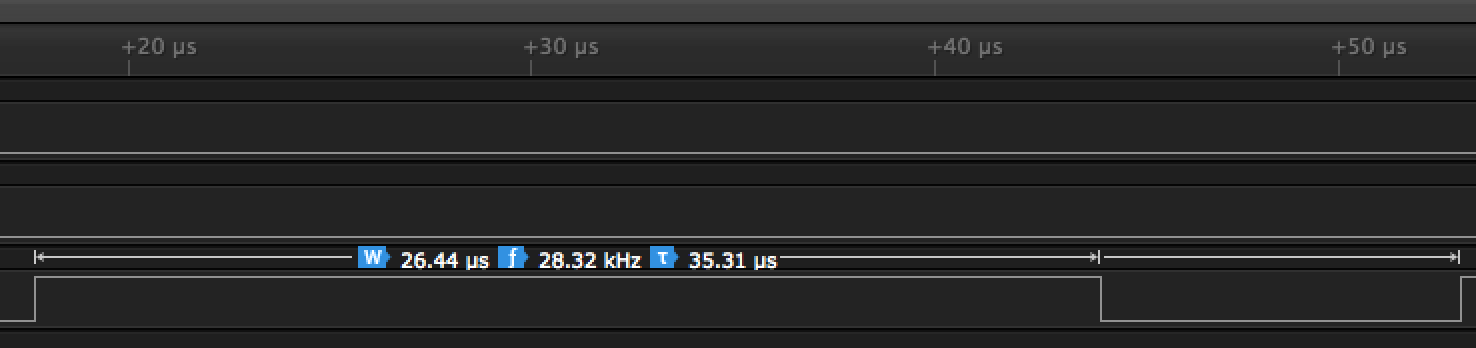
\includegraphics[width=0.5\textwidth]{resources/logic_fast_blinking.png}
		\caption{Выходной сигнал часто мигающей программы}
	\end{figure}
\end{frame}
\end{document}
